\chapter{Rates of reactions}
\section{Order, rate equation and rate reactions}
\subsection{Rate of reaction}
\paragraph{Rate of reaction is measured} by observing \textbf{changes over time}. It is basically measuring quantity produced/time e.g. cm$^3 s^{-1} $. In this chapter, you will mainly be dealing with concentration, so knowing the standard unit for it is important(mol $ dm^{-3}$).
\paragraph{Chemists use shorthand} to describe the concentration of compounds. This notation is [A], where A is the compound, and the square brackets mean 'concentration of'.
\begin{equation}
Rate \propto [A]^n - \textnormal{rate is directly proportional to the concentration of A}
\end{equation}
\subsection{Orders of reaction}
\paragraph{The rate of reaction}will often increase as the concentration is increased. It is directly proportional to the concentration raised to a power i.e.
\begin{equation}
rate\propto [A]^n
\end{equation}
The power is the order of reaction with respect to the concentration of the compound in the square brackets.
\subsubsection{Zero order}
\paragraph{This is when}\ch{rate=[A]^0}, meaning that a change in concentration has no effect on the rate of reaction. This is due to anything to the power of 0=1. 
\subsubsection{First order}
\paragraph{This is when}\ch{rate=[A]^1}. Essentially, what happens to the concentration happens to the rate i.e. concentration x2 means rate x2.
\subsubsection{Second order}
\paragraph{This is when}\ch{rate=[A]^2}.So when concentration doubles, rate x$2^2=4$. Basically the rate is the square of the change in concentration.
\subsection{Rate equation and rate constant}
\paragraph{The rate equation is}$rate=k[A]^n[B]^m$. The overall order can be found by adding the powers together. When a question says both concentrations are changed, you use the overall order to find the rate.
\paragraph{The units of the rate constant}are usually \ch{moldm^{-3}s^{-1}}. However,this can be derived by rearranging the rate equation to make k the subject as this is the rate constant. It is useful to remember that the concentrations are measured in \ch{moldm^{-3}}.
\subsection{Determining orders from experimental results}
\paragraph{The best way}to learn this is by doing past paper question. Some great resources can be found on: pastpapers.com; physicsandmathstutor.co.uk or http://www.a-levelchemistry.co.uk/.
\paragraph{The questions}will usually contain a table with the headings: Experiment, Concentration of respective elements and the initial rate. The way to go about these questions is by first seeing how the concentration change between experiments e.g. x2. Then look at initial rate. See how this changes to determine the rate e.g. if it's x4, this would be second order.
\begin{center}
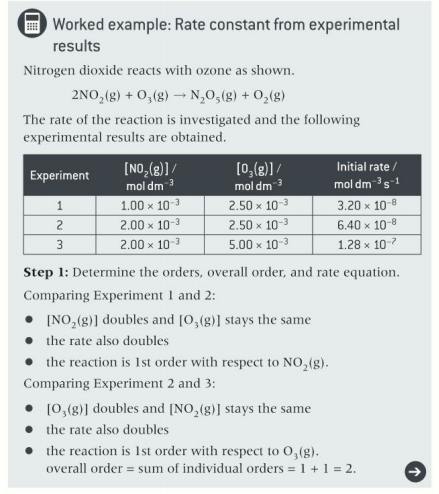
\includegraphics[scale=0.5]{workedorder.png}
\end{center}
\newpage
\section{Concentration-time graph}
\paragraph{You can measure rates}by looking for a \textbf{change} in mass or by gas collection in a certain \textbf{time}. You can also use a colorimeter if some of the compounds are coloured.
\subsection{Concentration-time graph}
\paragraph{The gradient of the concentration-time graph} is the rate of reaction.The order of reaction can be deduced from the shape of the graph.
\subsubsection{Zero order}
\paragraph{This graph slopes down}i.e. it has a negative gradient. The line is straight meaning that the rate is constant as concentration falls over time(as reactants used up). The gradient of the line is the rate constant-k.
\subsubsection{First order}
\paragraph{This graph is a downward-sloping curve}.The gradient decreases over time,slowing the reaction down. The \textbf{half-life}( \textit{time taken for concentration to halve}) is constant.
(INSERT GRAPHS WHEN BOTHERED)
\subsubsection{Second order}
\paragraph{This graph is steeper at the beginning than the first order.}However, it tails off more slowly
\subsection{Half-life}
\paragraph{Half-life,}which can be represented by $t_{1/2}$ is the time taken for half of the reactant to be used up. First order reactions halve the concentration every half life. The curve is exponential, showing \textbf{exponential decay}
\subsubsection{Determination of rate constant from rate}
\paragraph{You can draw a tangent to the curve}on a concentration-time graph.This will give you the rate of reaction. Then, you insert this into your re-arranged rate equation,where k is the subject.This should give you the rate constant, all you need to do is figure out the units.
\paragraph{You can also use an awesome formula:}\begin{equation}
k=\frac{\textnormal{ln}2}{t_{1/2}}
\end{equation}
This method is more accurate than drawing a tangent.
\section{Rate-concentration graphs and initial rates}
\paragraph{Always be careful to check the axes of your graph.}Here, the rate is on the left and concentration along the bottom. Normally, as concentration increases, so does rate due to kinetics i.e. more particles etc. Therefore the curves usually\textbf{slope up} rather than down.
\subsection{Orders from shapes}
\subsubsection{Zero order}
\paragraph{The gradient is 0,}meaning there is no slope. Rate is not affected by a change in concentration( a visual representation of its definition).The y-intercept gives you the rate constant-k.
\subsubsection{First order}
\paragraph{This is a upward-sloping straight-line graph}beginning at the origin. This is because when concentration is 0, rate is zero. The rate constant her is the gradient of the line.
\subsubsection{Second order}
\paragraph{This is an upward sloping curve.}Therefore the gradient constantly increases. It also means that the rate constant cannot be worked out directly by the curve. Instead, you need to \textbf{plot a second graph} of the rate against $[A]^2$ (concentration squared). This will give you a straight line graph through the origin, where the gradient is k.
\subsection{Initial rates method}
\paragraph{The initial rate}is the instantaneous rate when t=0.It can be measured by drawing a tangent where t=0 on a concentration-time graph.
\paragraph{A clock reaction}is a more convenient method of obtaining the initial rate. It is done by measuring time from the beginning of an experiment to a visual change. this will often be a precipitate or colour.
=======
\chapter{Physical chemistry and transition elements}

